\documentclass[11pt,oneside,leqno]{article}
\usepackage[paperwidth=6.5in,paperheight=9.5in,margin=.72in]{geometry}
\usepackage{fontspec}
\setmainfont{lmroman10-regular.otf}[BoldFont=lmroman10-bold.otf,ItalicFont=lmroman10-italic.otf,BoldItalicFont=lmroman10-bolditalic.otf,SmallCapsFont=lmromancaps10-regular.otf]
\usepackage[english]{babel}
\usepackage{amsmath,amssymb,microtype,needspace,multirow,booktabs,tikz}
\usepackage[unicode,hidelinks]{hyperref}
\hypersetup{pdftitle={Problems and theorems in elementary geometry},pdfauthor={Carl Friedrich Gauss}}
\newcommand{\SourceLeaf}[1]{\hypertarget{native-#1}{}}
\newcommand{\BareRoot}[1]{\mathord{\surd}#1}
\setlength{\parindent}{1.2em}
\setlength{\emergencystretch}{1.4em}
\widowpenalty=10000\clubpenalty=10000\raggedbottom
\newcommand{\HistoricalNote}[3]{\begingroup\renewcommand{\thefootnote}{#1}\footnotemark\renewcommand{\thefootnote}{#2}\footnotetext{#3}\endgroup}
\makeatletter
\long\def\@makefntext#1{\parindent1em\noindent\hb@xt@2.4em{\hss\@thefnmark\ }#1}
\makeatother
\newcommand{\EqualsOverGreater}{\mathrel{\vcenter{\offinterlineskip\hbox{$=$}\kern1pt\hbox{$>$}}}}
\newfontfamily\CyrillicFont{Times New Roman}
\newcommand{\gausscyr}[1]{{\CyrillicFont #1}}
\newcommand{\TripleParallel}{\mathrel{\rotatebox{-12}{$\vert$}\mkern-2mu\rotatebox{-12}{$\vert$}\mkern-2mu\rotatebox{-12}{$\vert$}}}
\begin{document}
\clearpage\SourceLeaf{294}
\thispagestyle{empty}
\vspace*{4cm}
\begin{center}
\textbf{\Large PROBLEMS AND THEOREMS}\par\medskip
\textbf{BELONGING TO}\par\medskip
\textbf{ELEMENTARY GEOMETRY.}\par\bigskip
SUPPLEMENTS TO VOLUME IV.
\end{center}
\clearpage
%
\SourceLeaf{296}
\begin{center}
\textbf{POSTHUMOUS PAPERS AND CORRESPONDENCE.}

\vspace{1em}

\textbf{[ON SPHERICAL TRIGONOMETRY.]}

\vspace{0.5em}

\end{center}

\vspace{1em}

\begin{center}[1.]\end{center}

\begin{center}
\textsc{Gauss} to \textsc{Gerling}. Göttingen, 18 February 1815.
\end{center}

Many thanks, dear \textsc{Gerling}, for what you have sent me from
your work on trigonometry. I find your proof of the 4 equations
quite appropriate for your purpose. All it needs for
completeness is a separate proof of the signs,
since, for\,example, from
\[
\sin \tfrac12 A^2 \cos \tfrac12 (b+c)^2 = \cos \tfrac12 (B+C)^2 \cos \tfrac12 a^2
\]
nothing actually follows except that
\[
\begin{array}{r@{\ }c@{\ }l}
\sin \tfrac12 A \cos \tfrac12 (b+c) & \text{either} & {}=\cos \tfrac12 (B+C) \cos \tfrac12 a \\[4pt]
 & \text{or} & {}=-\cos \tfrac12 (B+C) \cos \tfrac12 a.
\end{array}
\]

One can derive such a completion of the proof from other propositions,
but that makes the whole considerably longer. Lately I have always followed
the following method of derivation.

I assume the 5 equations, since in fact they are all needed
in any case.
%
\SourceLeaf{297}
\[
\begin{aligned}
1) \quad & \cos a = \cos b \cos c + \sin b \sin c \cos A \\
2) \quad & \sin a \cos B = \cos b \sin c - \sin b \cos c \cos A \\
3) \quad & \sin a \sin B = \sin b \sin A \\
4) \quad & \cos B \sin C + \sin B \cos C \cos a = \cos b \sin A \\
5) \quad & -\cos B \cos C + \sin B \sin C \cos a = \cos A.
\end{aligned}
\]

From these you can readily derive the following 6 new equations
\[
\left.\begin{aligned}
6) \quad & \sin a(\cos C - \cos B) = (1+\cos A)\sin(b-c) \\
7) \quad & \sin a(\cos C + \cos B) = (1-\cos A)\sin(b+c)
\end{aligned}\right\}\ \text{from 2),}
\]
\[
\left.\begin{aligned}
8) \quad & \sin A(\sin b + \sin c) = \sin a(\sin B + \sin C) \\
9) \quad & \sin A(\sin b - \sin c) = \sin a(\sin B - \sin C)
\end{aligned}\right\}\ \text{from 3),}
\]
\[
\left.\begin{aligned}
10) \quad & \sin A(\cos c + \cos b) = (1+\cos a)\sin(B+C) \\
11) \quad & \sin A(\cos c - \cos b) = (1-\cos a)\sin(B-C)
\end{aligned}\right\}\ \text{from 4).}
\]

[Here one uses equation 2)] partly in its original form
and partly by interchanging $B$, $b$ with $C$, $c$. The same applies to the
following [equations 3) and 4)].

If one now factors everything and, to save
writing, sets
\[
\begin{array}{ll}
\cos \tfrac12 A \cos \tfrac12 (b-c) = P & \cos \tfrac12 a \cos \tfrac12 (B+C) = p \\[4pt]
\cos \tfrac12 A \sin \tfrac12 (b-c) = Q & \cos \tfrac12 a \sin \tfrac12 (B+C) = q \\[4pt]
\sin \tfrac12 A \cos \tfrac12 (b+c) = R & \sin \tfrac12 a \cos \tfrac12 (B-C) = r \\[4pt]
\sin \tfrac12 A \sin \tfrac12 (b+c) = S & \sin \tfrac12 a \sin \tfrac12 (B-C) = s,
\end{array}
\]
the last 6 equations take the following form.
\[
\begin{aligned}
6^\ast) \quad & PQ = qs \\
7^\ast) \quad & RS = pr \\
8^\ast) \quad & PS = qr \\
9^\ast) \quad & QR = ps \\
10^\ast) \quad & PR = pq \\
11^\ast) \quad & QS = rs.
\end{aligned}
\]
%
\SourceLeaf{298}
From $\dfrac{6^\ast\times 8^\ast}{11^\ast}$ or $\dfrac{6^\ast\times 10^\ast}{9^\ast}$ or $\dfrac{8^\ast\times 10^\ast}{7^\ast}$ it follows that

\[
PP=qq,
\]

from which one must necessarily conclude that

\[
P=+q
\]

provided one considers only triangles whose sides and angles do not exceed $180^0$. Then one has immediately

\[
Q=+s,\qquad R=+p,\qquad S=+r,
\]

which together are the four desired propositions.

I leave it to you to decide how much use to make in your work of this or of my other customary ways of arranging calculations. \mbox{.\,.\,.}

\medskip

\Needspace{8\baselineskip}
\begin{center}
[2.]

\textsc{Gauss} to \textsc{Gerling}. Göttingen, 26 June 1816.
\end{center}

\mbox{.\,.\,.\,.\,.\,.\,.} I have been so constantly distracted by various matters that I have not yet got around to considering the most suitable order for the first propositions of spherical trigonometry in a geometrical treatment. I should think, however, that it would be simplest to take Euclid XI. 20. 21 as the basis and to derive the proposition that $A+B+C>180^0$ from the polar triangle. I scarcely think that any substantial advantage can be gained by considering the plane triangle formed by the vertices of the spherical one, since there do not seem to be any \textls{very} simple relations among its angles. The following may well be one of the most elegant. If $A'$, $B'$, $C'$ are the angles of the plane triangle and

\[
A+B+C-180^0=u,
\]

then

\[
\cos A'=\cos\tfrac{1}{2}a\cos(A-\tfrac{1}{2}u).
\]

\mbox{.\,.\,.\,.\,.\,.\,.\,.\,.}
%
\clearpage\SourceLeaf{299}
\begin{center}
\textbf{[LOCUS}\par\medskip
\textbf{OF THE APEX OF A SPHERICAL TRIANGLE}\par\medskip
\textbf{ON A GIVEN BASE WITH A GIVEN AREA.]}
\end{center}

\medskip

\begin{center}
\textsc{Gauss} to \textsc{Schumacher}. Göttingen, 29 December 1841.
\end{center}

\mbox{.\,.\,.\,.\,.\,.\,.} Do you know of a \textls{printed} solution to the problem of finding the locus of the apex of a spherical triangle on a given base and with a given area? I recently had occasion to look for one and was somewhat surprised that the analytical solution leads by a somewhat roundabout route to a very simple result whose synthetic proof can be given in a few lines. \mbox{.\,.\,.\,.\,.\,.\,.}

\medskip

\begin{center}
[\textsc{Schumacher} \emph{to} \textsc{Gauss}.\ \emph{Altona, 3 January 1842.}]
\end{center}

\{A geometrical solution to the problem you mentioned, my dearest friend, was given not very long ago by \textsc{Steiner} in \textsc{Crelle}'s journal (vol.\ 2.\ p.\ 45), where he does not cite his predecessors correctly. \textsc{Lexell}'s paper is not in Nova Acta Petrop.\ V.\ Pars 1, as stated there. It is in Acta Petrop.\ pro 1781, Pars I. \textsc{Euler} returned to it later in Nova Acta Tom.\ X.\ p.\ 47 (Variae speculationes etc.). \textsc{Legendre} has it
%
\SourceLeaf{300}
also in his Géométrie, Note X, where he too cites \textsc{Lexell} incorrectly, and \textsc{Grunert} has it in the continuation of \textsc{Klügel}'s Wörterbuch, article Trigonometrie (likewise an incorrect citation of \textsc{Lexell}. They seem to have copied from \textsc{Legendre}).

\textsc{Clausen} has asked me to present his solution to you. His solution shows that the midpoints of the other two sides of the triangle (the base is the third) lie on great circles. The following simple construction gives the pole of the locus circle.

\begin{quote}
Bisect the other two sides and let arcs of $90^0$ from the points of bisection intersect. Their intersection is the required pole of the small circle on which the apices of the triangles lie.
\end{quote}

Has this already been found by geometrical reasoning? \mbox{.\,.\,.\,.\,.\,.\,.\,.}\}

\medskip

\Needspace{6\baselineskip}
\begin{center}
\textsc{Gauss} to \textsc{Schumacher}. Göttingen, 6 January 1842.
\end{center}

\mbox{.\,.\,.\,.\,.\,.\,.} The only thing that struck me about the whole matter was that this time the analytical work of tackling it is much longer than the synthetic proof once the theorem is known. I myself had stated the result as follows. Join the midpoints of the two sides of the given triangle (calling the given base the third side) by a great circle. The small circle drawn parallel to it through the apex of the triangle is the required locus. One can see at once that this solves the problem.

\Needspace{20\baselineskip}
\begin{center}\resizebox{7.3cm}{!}{%
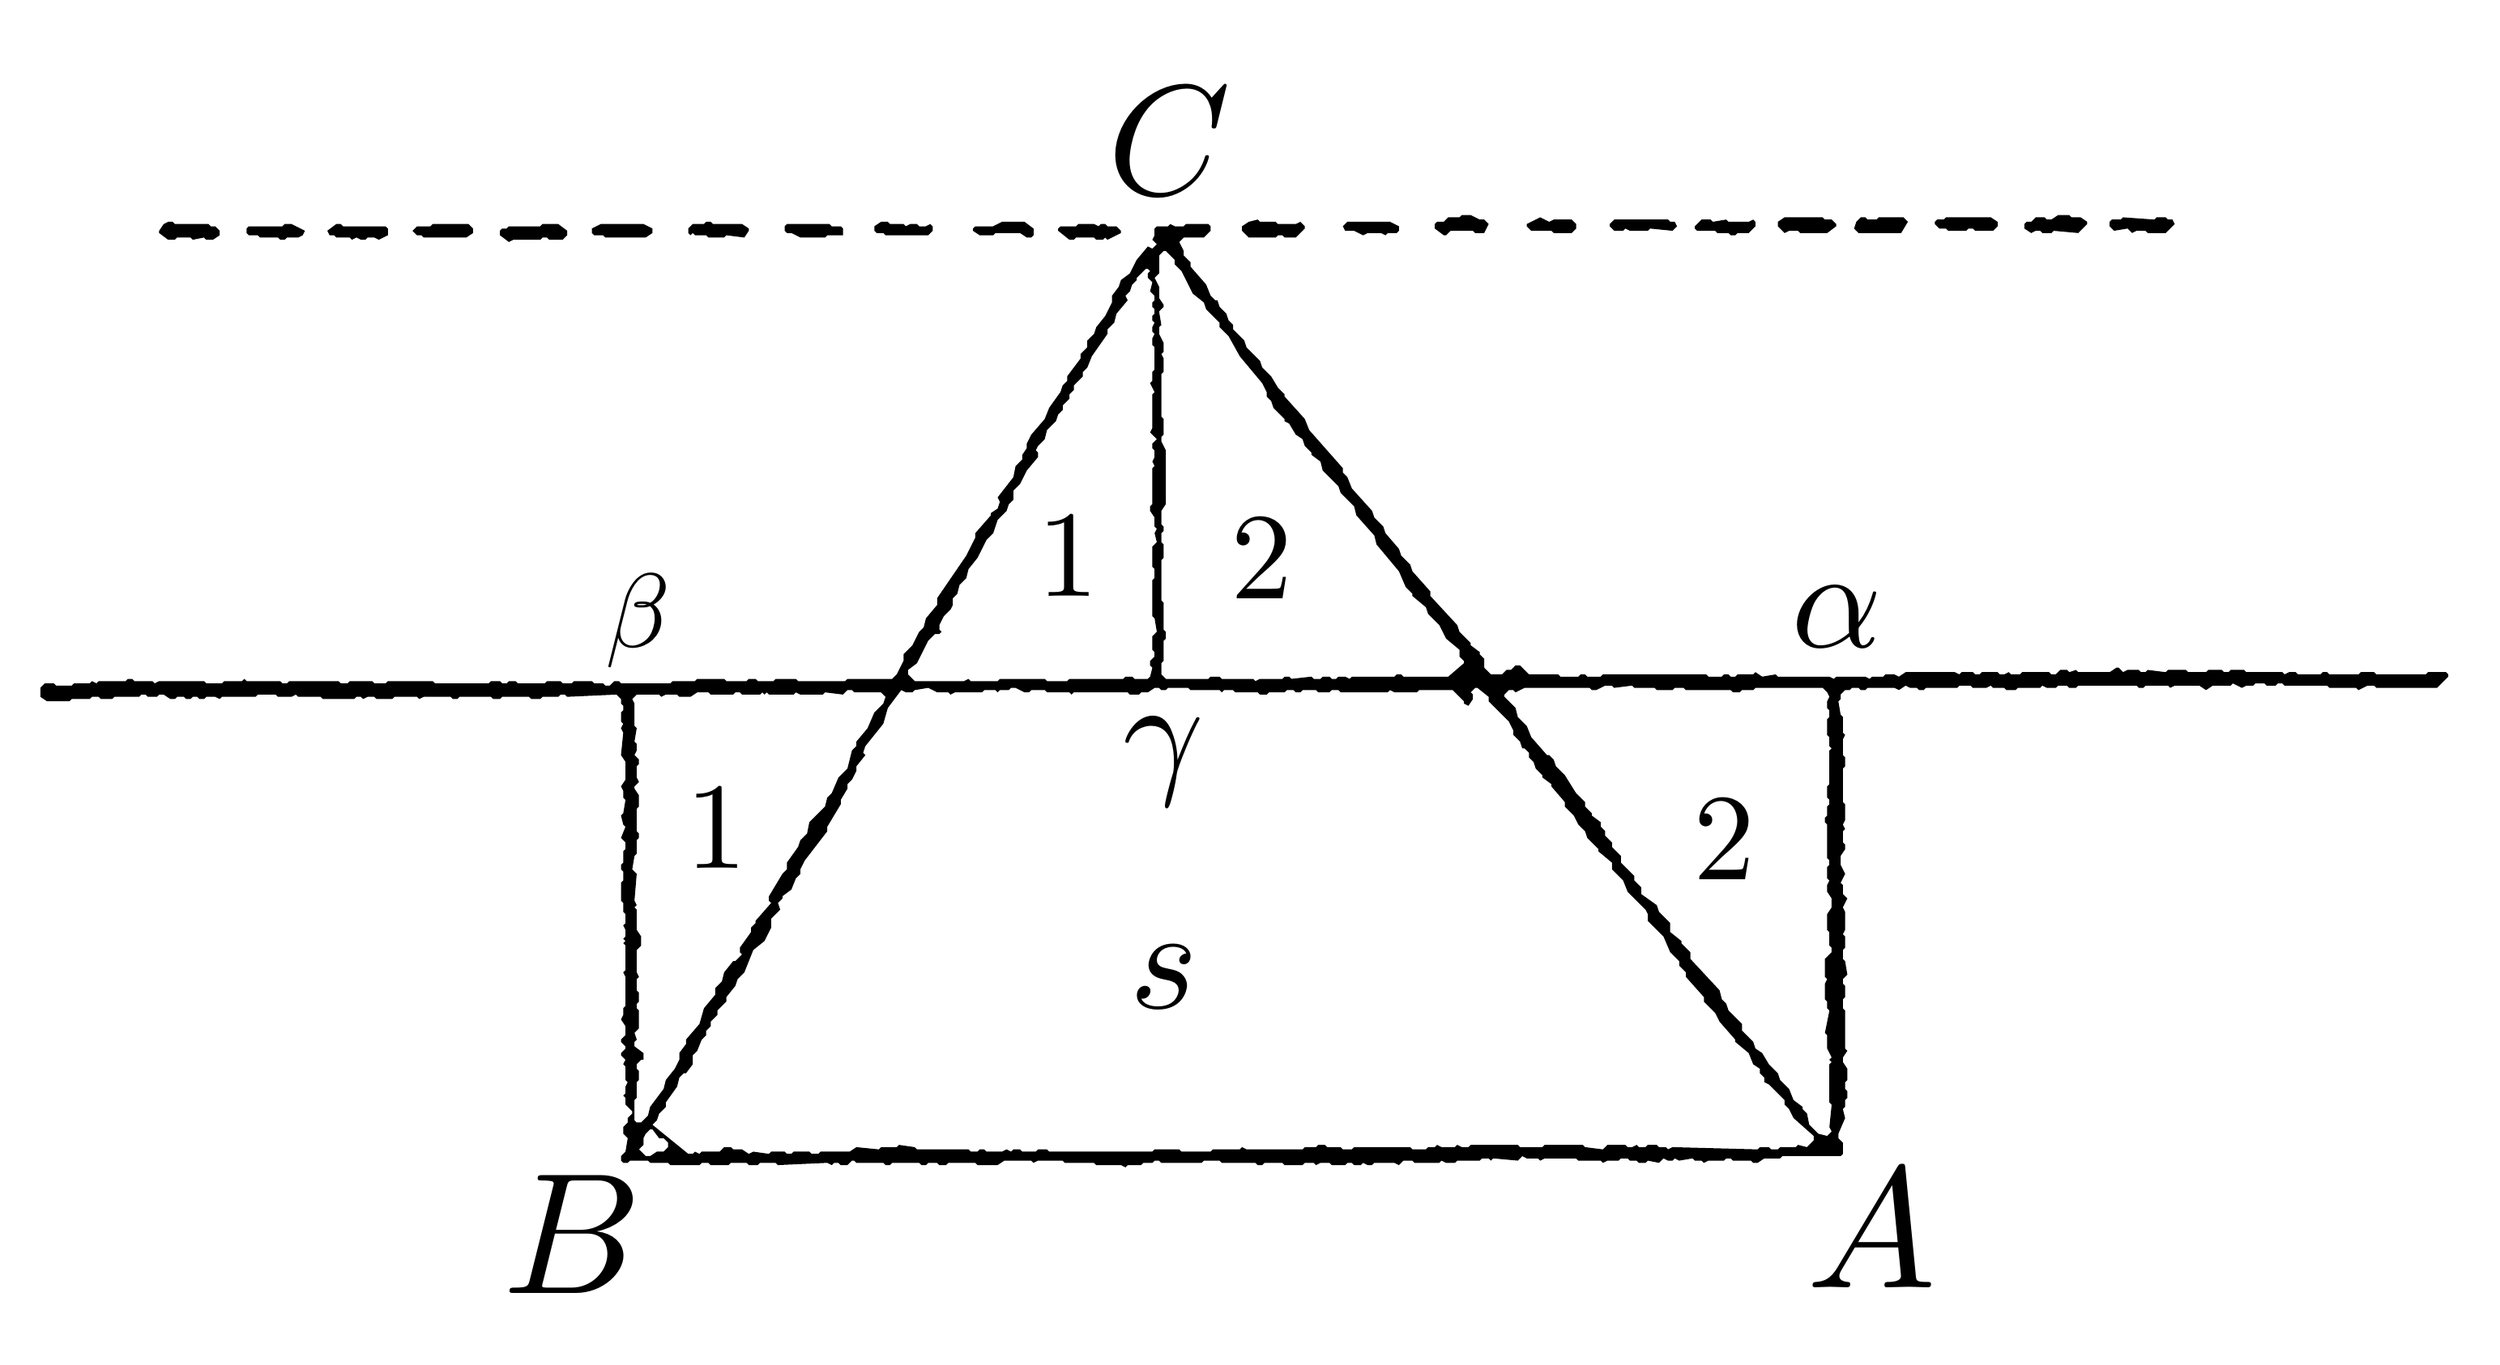
\begin{tikzpicture}[x=1pt,y=-1pt]
\path[use as bounding box] (0,0) rectangle (1095,589);
\path[fill=black,draw=none,even odd rule]
(8,301) -- (11,303) -- (21,303) -- (22,302) -- (30,302) -- (31,301) -- (34,301) -- (35,302) -- (40,302) -- (41,301) -- (52,301) -- (53,300) -- (55,300) -- (56,301) -- (60,301) -- (61,300) -- (63,300) -- (66,302) -- (68,302) -- (69,301) -- (72,301) -- (73,302) -- (75,302) -- (76,301) -- (78,301) -- (79,302) -- (81,302) -- (82,301) -- (86,301) -- (88,302) -- (89,301) -- (104,301) -- (105,300) -- (113,300) -- (114,301) -- (120,301) -- (122,300) -- (123,301) -- (133,301) -- (134,302) -- (148,302) -- (149,301) -- (151,301) -- (152,302) -- (154,301) -- (157,301) -- (158,302) -- (165,302) -- (166,301) -- (176,301) -- (177,302) -- (179,301) -- (191,301) -- (192,302) -- (194,302) -- (195,301) -- (209,301) -- (210,302) -- (213,302) -- (214,301) -- (226,301) -- (227,302) -- (231,302) -- (232,301) -- (239,301) -- (240,300) -- (242,300) -- (243,301) -- (265,300) -- (267,302) -- (267,304) -- (268,305) -- (268,307) -- (267,308) -- (267,312) -- (268,313) -- (267,315) -- (268,317) -- (267,327) -- (269,330) -- (269,338) -- (267,341) -- (268,343) -- (268,346) -- (269,347) -- (268,353) -- (267,354) -- (268,358) -- (269,359) -- (267,364) -- (269,366) -- (269,369) -- (268,370) -- (268,375) -- (267,376) -- (267,378) -- (268,379) -- (268,383) -- (267,384) -- (267,392) -- (268,393) -- (268,397) -- (269,398) -- (269,402) -- (268,403) -- (269,405) -- (269,408) -- (268,409) -- (269,410) -- (268,411) -- (269,412) -- (269,423) -- (268,424) -- (269,426) -- (269,439) -- (268,440) -- (268,443) -- (267,445) -- (269,448) -- (269,452) -- (267,454) -- (267,455) -- (269,457) -- (269,458) -- (267,460) -- (267,461) -- (269,463) -- (268,465) -- (269,466) -- (269,472) -- (270,473) -- (269,475) -- (269,478) -- (268,479) -- (269,480) -- (269,483) -- (272,486) -- (272,487) -- (270,489) -- (270,491) -- (268,493) -- (268,496) -- (270,498) -- (269,504) -- (267,506) -- (267,508) -- (268,509) -- (270,509) -- (271,508) -- (279,508) -- (280,509) -- (288,509) -- (289,510) -- (302,510) -- (303,509) -- (306,509) -- (307,510) -- (315,510) -- (316,509) -- (323,509) -- (324,510) -- (328,510) -- (329,509) -- (336,509) -- (337,510) -- (359,509) -- (361,510) -- (362,509) -- (364,509) -- (365,510) -- (368,510) -- (370,508) -- (371,508) -- (372,509) -- (384,509) -- (385,510) -- (387,510) -- (388,509) -- (400,509) -- (401,510) -- (403,510) -- (404,509) -- (408,509) -- (409,510) -- (412,510) -- (413,509) -- (425,509) -- (426,510) -- (435,510) -- (438,508) -- (450,508) -- (451,509) -- (453,508) -- (464,508) -- (465,509) -- (478,509) -- (479,510) -- (490,510) -- (492,511) -- (493,510) -- (499,510) -- (500,509) -- (504,509) -- (505,508) -- (507,508) -- (508,509) -- (526,509) -- (527,508) -- (534,508) -- (535,509) -- (550,509) -- (551,510) -- (553,510) -- (554,509) -- (562,509) -- (563,510) -- (571,510) -- (572,509) -- (576,509) -- (577,510) -- (579,509) -- (583,509) -- (584,510) -- (590,510) -- (591,509) -- (593,509) -- (594,510) -- (597,510) -- (598,509) -- (600,510) -- (602,510) -- (603,509) -- (612,509) -- (614,510) -- (616,508) -- (620,508) -- (621,509) -- (632,509) -- (633,508) -- (635,509) -- (639,509) -- (640,508) -- (650,508) -- (651,507) -- (654,507) -- (655,508) -- (656,507) -- (667,508) -- (669,506) -- (671,507) -- (676,507) -- (677,508) -- (679,507) -- (693,507) -- (694,508) -- (704,508) -- (705,509) -- (707,508) -- (712,508) -- (713,507) -- (716,507) -- (717,508) -- (720,508) -- (721,509) -- (724,509) -- (725,508) -- (730,509) -- (732,507) -- (734,508) -- (736,508) -- (737,507) -- (739,508) -- (745,507) -- (746,508) -- (749,508) -- (750,509) -- (752,508) -- (759,508) -- (760,507) -- (762,507) -- (763,508) -- (771,508) -- (772,509) -- (774,509) -- (777,507) -- (784,507) -- (785,506) -- (811,506) -- (812,505) -- (812,500) -- (810,498) -- (810,496) -- (813,489) -- (812,485) -- (813,484) -- (813,481) -- (814,480) -- (814,477) -- (813,476) -- (813,473) -- (814,472) -- (814,467) -- (812,464) -- (812,462) -- (814,459) -- (813,458) -- (813,441) -- (812,440) -- (812,436) -- (813,435) -- (813,430) -- (812,429) -- (812,427) -- (814,425) -- (813,419) -- (812,418) -- (812,414) -- (813,413) -- (813,408) -- (812,407) -- (813,405) -- (813,397) -- (812,395) -- (814,391) -- (812,389) -- (812,385) -- (811,384) -- (813,380) -- (811,376) -- (811,372) -- (813,369) -- (813,367) -- (812,366) -- (812,361) -- (813,360) -- (812,358) -- (813,356) -- (813,349) -- (812,348) -- (812,333) -- (813,332) -- (813,328) -- (812,327) -- (812,320) -- (813,318) -- (812,317) -- (812,310) -- (811,309) -- (810,303) -- (811,302) -- (811,300) -- (813,298) -- (815,298) -- (816,297) -- (819,297) -- (820,298) -- (822,298) -- (823,297) -- (835,297) -- (837,298) -- (840,296) -- (842,297) -- (845,297) -- (846,298) -- (848,298) -- (849,297) -- (863,297) -- (864,296) -- (869,296) -- (870,297) -- (876,297) -- (878,296) -- (879,297) -- (884,297) -- (885,298) -- (889,298) -- (890,297) -- (900,297) -- (901,296) -- (903,297) -- (907,297) -- (908,296) -- (912,296) -- (913,297) -- (916,297) -- (917,296) -- (943,296) -- (944,297) -- (946,297) -- (947,296) -- (957,296) -- (958,297) -- (960,296) -- (971,296) -- (974,298) -- (977,296) -- (985,296) -- (986,295) -- (990,297) -- (992,296) -- (995,296) -- (996,295) -- (1000,295) -- (1001,296) -- (1005,296) -- (1006,295) -- (1008,295) -- (1009,296) -- (1028,296) -- (1029,297) -- (1041,297) -- (1042,298) -- (1046,296) -- (1049,296) -- (1050,297) -- (1077,297) -- (1082,292) -- (1082,291) -- (1081,290) -- (1073,290) -- (1072,291) -- (1050,291) -- (1049,290) -- (1043,290) -- (1042,291) -- (1029,291) -- (1028,290) -- (1026,290) -- (1025,291) -- (1015,291) -- (1014,290) -- (1011,290) -- (1009,291) -- (1008,290) -- (992,290) -- (991,289) -- (985,289) -- (984,290) -- (982,290) -- (981,289) -- (975,289) -- (974,290) -- (966,290) -- (965,289) -- (957,289) -- (956,290) -- (948,289) -- (947,290) -- (945,290) -- (944,289) -- (939,289) -- (937,290) -- (935,288) -- (934,288) -- (931,290) -- (917,290) -- (916,289) -- (913,290) -- (912,289) -- (909,289) -- (907,291) -- (905,291) -- (904,290) -- (892,290) -- (891,291) -- (887,291) -- (886,290) -- (884,291) -- (882,291) -- (881,290) -- (874,290) -- (873,291) -- (871,291) -- (870,290) -- (865,290) -- (864,291) -- (862,290) -- (840,290) -- (837,292) -- (835,291) -- (831,291) -- (830,292) -- (825,292) -- (824,293) -- (822,292) -- (809,292) -- (808,293) -- (806,292) -- (783,292) -- (782,291) -- (776,292) -- (773,290) -- (772,291) -- (765,291) -- (764,292) -- (762,292) -- (761,291) -- (759,291) -- (758,292) -- (752,292) -- (751,291) -- (705,291) -- (704,292) -- (698,292) -- (697,291) -- (695,291) -- (694,292) -- (686,292) -- (685,291) -- (672,291) -- (668,287) -- (666,287) -- (664,289) -- (662,289) -- (660,291) -- (655,291) -- (652,288) -- (652,284) -- (650,282) -- (650,281) -- (646,278) -- (646,277) -- (641,272) -- (640,269) -- (628,256) -- (628,254) -- (620,245) -- (619,242) -- (615,238) -- (614,235) -- (608,228) -- (607,225) -- (603,221) -- (602,218) -- (593,208) -- (591,203) -- (589,201) -- (589,199) -- (574,182) -- (572,177) -- (563,167) -- (563,166) -- (560,163) -- (557,158) -- (553,154) -- (552,151) -- (546,145) -- (545,142) -- (540,137) -- (540,135) -- (538,133) -- (537,130) -- (534,127) -- (533,124) -- (532,124) -- (530,122) -- (528,117) -- (521,109) -- (521,107) -- (518,104) -- (518,102) -- (516,98) -- (518,96) -- (527,96) -- (530,93) -- (530,91) -- (529,90) -- (519,90) -- (518,91) -- (514,91) -- (512,90) -- (511,91) -- (506,91) -- (505,92) -- (505,95) -- (504,97) -- (506,99) -- (504,101) -- (502,100) -- (497,106) -- (494,112) -- (490,115) -- (489,118) -- (486,122) -- (486,125) -- (483,131) -- (479,136) -- (478,139) -- (475,142) -- (475,145) -- (472,148) -- (472,150) -- (466,158) -- (466,160) -- (464,162) -- (463,165) -- (458,172) -- (456,177) -- (450,184) -- (448,188) -- (448,190) -- (446,193) -- (446,195) -- (443,198) -- (442,203) -- (435,212) -- (436,214) -- (435,217) -- (432,219) -- (432,220) -- (425,228) -- (425,230) -- (421,238) -- (408,257) -- (408,260) -- (403,266) -- (402,270) -- (400,272) -- (397,278) -- (393,282) -- (393,285) -- (390,291) -- (388,293) -- (368,293) -- (367,294) -- (346,294) -- (345,293) -- (336,293) -- (335,294) -- (328,294) -- (327,293) -- (324,293) -- (323,294) -- (314,294) -- (313,293) -- (301,293) -- (300,294) -- (290,294) -- (289,295) -- (267,295) -- (266,294) -- (264,294) -- (262,296) -- (260,296) -- (259,295) -- (255,295) -- (254,294) -- (246,294) -- (245,295) -- (241,295) -- (240,294) -- (234,294) -- (233,295) -- (221,295) -- (220,294) -- (217,294) -- (216,295) -- (214,295) -- (213,294) -- (209,294) -- (208,295) -- (184,295) -- (183,294) -- (163,294) -- (162,295) -- (157,295) -- (156,294) -- (146,294) -- (145,295) -- (142,295) -- (141,294) -- (119,294) -- (118,295) -- (116,295) -- (115,294) -- (100,294) -- (99,293) -- (98,294) -- (90,294) -- (89,295) -- (82,295) -- (81,294) -- (61,294) -- (59,295) -- (58,294) -- (50,294) -- (49,293) -- (47,293) -- (46,294) -- (34,294) -- (33,295) -- (31,294) -- (30,295) -- (23,295) -- (22,296) -- (15,296) -- (14,295) -- (10,295) -- (8,297) -- cycle
(281,494) -- (284,498) -- (286,498) -- (288,500) -- (288,502) -- (286,504) -- (283,504) -- (280,506) -- (278,506) -- (275,503) -- (277,501) -- (277,498) -- (278,496) -- (280,494) -- cycle
(383,299) -- (385,301) -- (384,304) -- (380,308) -- (377,315) -- (372,321) -- (372,323) -- (370,325) -- (368,333) -- (364,337) -- (361,344) -- (359,346) -- (358,350) -- (351,357) -- (350,362) -- (347,365) -- (346,368) -- (341,375) -- (341,378) -- (339,380) -- (333,390) -- (333,392) -- (334,393) -- (327,401) -- (327,402) -- (325,404) -- (325,406) -- (320,413) -- (320,415) -- (321,416) -- (318,419) -- (317,419) -- (313,424) -- (312,428) -- (309,431) -- (309,434) -- (304,440) -- (302,447) -- (296,454) -- (296,456) -- (293,460) -- (293,463) -- (291,467) -- (287,472) -- (286,476) -- (280,484) -- (279,488) -- (276,491) -- (274,491) -- (273,490) -- (273,481) -- (274,480) -- (274,473) -- (275,472) -- (275,468) -- (274,467) -- (274,465) -- (276,463) -- (277,463) -- (277,460) -- (273,457) -- (273,455) -- (274,454) -- (273,451) -- (275,449) -- (275,441) -- (274,440) -- (274,438) -- (275,437) -- (275,433) -- (274,432) -- (274,427) -- (275,426) -- (274,424) -- (274,414) -- (276,412) -- (276,408) -- (274,405) -- (274,396) -- (273,395) -- (274,394) -- (273,392) -- (274,380) -- (272,378) -- (273,372) -- (274,371) -- (274,365) -- (275,364) -- (275,362) -- (274,361) -- (274,351) -- (275,350) -- (275,345) -- (273,342) -- (273,341) -- (275,339) -- (274,337) -- (274,332) -- (275,331) -- (275,329) -- (273,327) -- (274,325) -- (274,322) -- (273,321) -- (274,315) -- (273,314) -- (273,304) -- (272,302) -- (274,300) -- (284,300) -- (285,301) -- (287,300) -- (292,300) -- (293,301) -- (298,301) -- (301,299) -- (306,299) -- (307,300) -- (317,300) -- (318,299) -- (320,299) -- (321,300) -- (329,300) -- (330,299) -- (331,300) -- (332,299) -- (333,300) -- (344,300) -- (345,299) -- (347,300) -- (357,300) -- (358,299) -- (366,300) -- (368,298) -- (370,298) -- (371,299) -- cycle
(281,492) -- (283,490) -- (284,487) -- (287,484) -- (287,482) -- (292,475) -- (293,471) -- (295,469) -- (296,469) -- (299,465) -- (299,461) -- (301,459) -- (303,454) -- (305,452) -- (305,450) -- (307,448) -- (307,446) -- (310,443) -- (310,441) -- (314,437) -- (314,435) -- (318,430) -- (319,427) -- (322,424) -- (326,414) -- (331,410) -- (334,404) -- (334,400) -- (338,396) -- (337,393) -- (339,391) -- (339,390) -- (343,387) -- (345,382) -- (347,380) -- (347,378) -- (349,374) -- (359,361) -- (359,359) -- (365,349) -- (365,347) -- (368,342) -- (368,340) -- (370,338) -- (372,334) -- (372,332) -- (376,327) -- (375,326) -- (376,323) -- (384,313) -- (386,306) -- (392,298) -- (394,299) -- (397,299) -- (398,298) -- (404,297) -- (408,299) -- (413,299) -- (414,300) -- (416,299) -- (428,299) -- (429,298) -- (434,298) -- (435,299) -- (436,298) -- (440,298) -- (441,297) -- (443,297) -- (447,299) -- (449,299) -- (450,298) -- (456,298) -- (457,299) -- (467,299) -- (468,300) -- (469,299) -- (493,299) -- (494,300) -- (498,300) -- (499,299) -- (502,299) -- (505,297) -- (507,297) -- (508,298) -- (510,298) -- (511,297) -- (520,297) -- (521,298) -- (534,298) -- (535,299) -- (536,298) -- (540,298) -- (541,299) -- (551,299) -- (552,300) -- (555,300) -- (556,299) -- (563,299) -- (564,298) -- (567,298) -- (568,299) -- (570,299) -- (571,298) -- (577,298) -- (578,299) -- (583,299) -- (584,298) -- (587,298) -- (588,299) -- (609,299) -- (610,298) -- (612,299) -- (622,299) -- (623,298) -- (638,298) -- (643,303) -- (643,304) -- (645,305) -- (647,302) -- (647,300) -- (646,299) -- (648,297) -- (649,297) -- (654,301) -- (654,303) -- (663,312) -- (665,316) -- (665,318) -- (668,321) -- (669,324) -- (670,324) -- (672,326) -- (672,328) -- (674,330) -- (675,333) -- (678,336) -- (678,337) -- (682,340) -- (682,341) -- (688,348) -- (688,350) -- (692,354) -- (694,358) -- (697,361) -- (698,364) -- (703,369) -- (703,370) -- (709,375) -- (709,378) -- (714,383) -- (716,388) -- (724,396) -- (725,398) -- (725,401) -- (732,408) -- (735,415) -- (739,419) -- (739,421) -- (742,424) -- (742,426) -- (750,435) -- (750,437) -- (755,442) -- (757,446) -- (764,454) -- (764,455) -- (770,460) -- (772,465) -- (775,467) -- (775,469) -- (777,471) -- (777,473) -- (779,474) -- (786,481) -- (786,483) -- (788,485) -- (790,489) -- (799,497) -- (799,499) -- (796,502) -- (792,501) -- (791,502) -- (784,502) -- (783,503) -- (780,503) -- (779,502) -- (775,502) -- (774,503) -- (736,502) -- (734,503) -- (733,502) -- (730,502) -- (729,501) -- (725,501) -- (724,502) -- (721,502) -- (720,501) -- (718,502) -- (716,502) -- (715,501) -- (707,501) -- (705,503) -- (697,502) -- (696,501) -- (679,501) -- (678,502) -- (668,502) -- (667,501) -- (646,501) -- (645,502) -- (642,502) -- (640,501) -- (639,502) -- (633,502) -- (631,501) -- (630,502) -- (627,502) -- (626,503) -- (620,503) -- (619,502) -- (594,502) -- (593,503) -- (589,503) -- (588,502) -- (582,502) -- (581,501) -- (578,501) -- (577,502) -- (572,502) -- (571,503) -- (546,503) -- (544,502) -- (543,503) -- (531,503) -- (530,504) -- (517,504) -- (516,503) -- (505,503) -- (504,504) -- (458,504) -- (457,503) -- (453,503) -- (452,504) -- (446,504) -- (445,503) -- (442,503) -- (441,504) -- (439,503) -- (437,504) -- (430,504) -- (429,503) -- (427,503) -- (426,504) -- (423,504) -- (422,503) -- (399,503) -- (398,502) -- (391,501) -- (390,502) -- (383,502) -- (382,503) -- (372,502) -- (369,504) -- (356,504) -- (355,505) -- (352,505) -- (351,504) -- (344,504) -- (343,505) -- (341,505) -- (340,504) -- (334,504) -- (333,505) -- (326,504) -- (324,505) -- (321,503) -- (317,503) -- (316,502) -- (313,502) -- (311,504) -- (303,504) -- (302,505) -- (300,504) -- (299,505) -- (297,505) -- cycle
(663,298) -- (665,298) -- (666,299) -- (670,297) -- (699,297) -- (700,298) -- (702,298) -- (706,296) -- (709,296) -- (710,297) -- (718,296) -- (719,297) -- (728,297) -- (729,298) -- (736,298) -- (737,297) -- (741,297) -- (742,298) -- (762,298) -- (763,299) -- (766,299) -- (767,298) -- (772,298) -- (773,297) -- (803,297) -- (805,299) -- (806,301) -- (805,303) -- (805,306) -- (806,307) -- (806,310) -- (805,311) -- (805,318) -- (806,319) -- (806,323) -- (807,324) -- (806,325) -- (806,340) -- (805,341) -- (805,346) -- (806,347) -- (806,349) -- (805,350) -- (805,354) -- (804,355) -- (804,357) -- (805,358) -- (805,373) -- (806,374) -- (806,376) -- (805,377) -- (805,382) -- (806,383) -- (805,385) -- (805,388) -- (807,391) -- (807,395) -- (805,398) -- (805,405) -- (806,406) -- (806,412) -- (807,413) -- (807,415) -- (804,418) -- (804,426) -- (805,427) -- (804,429) -- (804,436) -- (805,437) -- (805,440) -- (806,441) -- (804,451) -- (805,452) -- (805,458) -- (807,462) -- (806,463) -- (807,464) -- (806,465) -- (806,482) -- (807,483) -- (806,493) -- (807,495) -- (805,497) -- (801,496) -- (797,492) -- (796,487) -- (794,485) -- (794,484) -- (790,481) -- (788,476) -- (784,472) -- (783,469) -- (779,465) -- (776,460) -- (773,458) -- (772,455) -- (767,450) -- (767,447) -- (761,441) -- (760,438) -- (758,436) -- (757,432) -- (744,418) -- (744,415) -- (740,411) -- (740,410) -- (735,406) -- (735,402) -- (730,397) -- (729,394) -- (722,389) -- (722,386) -- (719,383) -- (719,381) -- (713,375) -- (713,372) -- (709,368) -- (709,366) -- (706,363) -- (706,361) -- (704,359) -- (704,357) -- (700,354) -- (700,353) -- (697,350) -- (697,348) -- (693,344) -- (688,336) -- (684,332) -- (683,329) -- (681,327) -- (680,327) -- (673,319) -- (671,314) -- (667,310) -- (666,306) -- (661,301) -- (661,300) -- cycle
(502,110) -- (503,111) -- (502,112) -- (502,114) -- (504,116) -- (503,120) -- (505,122) -- (505,124) -- (504,125) -- (504,127) -- (505,128) -- (505,130) -- (504,131) -- (504,133) -- (505,134) -- (504,136) -- (504,138) -- (505,139) -- (504,141) -- (504,144) -- (505,145) -- (505,155) -- (504,156) -- (504,160) -- (503,161) -- (505,165) -- (504,166) -- (504,181) -- (503,183) -- (506,186) -- (504,188) -- (504,190) -- (505,191) -- (505,194) -- (504,196) -- (505,198) -- (504,199) -- (504,215) -- (503,216) -- (503,218) -- (505,221) -- (505,225) -- (506,226) -- (505,228) -- (506,232) -- (504,234) -- (504,243) -- (505,244) -- (505,248) -- (504,249) -- (504,265) -- (505,266) -- (506,272) -- (504,274) -- (504,280) -- (505,281) -- (505,283) -- (503,285) -- (503,287) -- (504,288) -- (503,292) -- (502,293) -- (496,293) -- (495,292) -- (492,292) -- (491,293) -- (467,293) -- (466,294) -- (457,294) -- (456,293) -- (436,293) -- (435,294) -- (423,294) -- (422,293) -- (420,294) -- (398,294) -- (395,291) -- (395,289) -- (399,286) -- (404,276) -- (407,273) -- (409,273) -- (410,272) -- (409,271) -- (409,269) -- (411,265) -- (414,262) -- (415,260) -- (415,257) -- (417,255) -- (418,251) -- (421,248) -- (422,244) -- (426,239) -- (430,231) -- (433,228) -- (435,222) -- (439,218) -- (440,215) -- (442,213) -- (442,209) -- (445,206) -- (448,200) -- (453,194) -- (453,192) -- (452,191) -- (453,189) -- (456,186) -- (457,182) -- (461,178) -- (462,175) -- (464,173) -- (464,171) -- (467,168) -- (467,166) -- (469,164) -- (469,162) -- (473,158) -- (473,156) -- (475,154) -- (477,149) -- (484,139) -- (484,137) -- (487,134) -- (488,130) -- (493,124) -- (492,122) -- (494,120) -- (495,117) -- (497,115) -- (497,114) -- (501,110) -- cycle
(509,102) -- (510,102) -- (514,106) -- (514,108) -- (517,111) -- (522,121) -- (527,125) -- (528,128) -- (534,134) -- (534,136) -- (538,140) -- (543,149) -- (553,161) -- (555,165) -- (555,167) -- (557,169) -- (558,172) -- (563,177) -- (563,178) -- (565,179) -- (568,184) -- (571,186) -- (572,189) -- (575,192) -- (575,193) -- (579,196) -- (580,200) -- (587,207) -- (588,210) -- (594,216) -- (595,220) -- (603,229) -- (604,233) -- (614,245) -- (617,252) -- (620,255) -- (620,256) -- (626,261) -- (627,264) -- (632,269) -- (635,275) -- (641,280) -- (641,283) -- (643,285) -- (643,286) -- (636,292) -- (616,292) -- (615,291) -- (613,291) -- (612,292) -- (593,292) -- (592,293) -- (590,292) -- (587,292) -- (586,293) -- (584,293) -- (583,292) -- (580,292) -- (579,293) -- (576,293) -- (575,292) -- (566,293) -- (565,292) -- (563,292) -- (562,293) -- (552,293) -- (550,294) -- (549,293) -- (535,293) -- (534,292) -- (530,292) -- (529,293) -- (510,293) -- (508,291) -- (508,286) -- (509,285) -- (509,276) -- (510,275) -- (510,272) -- (509,271) -- (509,259) -- (508,258) -- (508,240) -- (509,239) -- (509,233) -- (508,232) -- (508,228) -- (509,227) -- (509,225) -- (508,224) -- (508,218) -- (510,215) -- (510,191) -- (508,187) -- (508,185) -- (509,184) -- (509,177) -- (508,176) -- (508,157) -- (509,156) -- (509,150) -- (508,148) -- (509,147) -- (509,143) -- (507,139) -- (507,136) -- (508,135) -- (507,129) -- (509,127) -- (509,126) -- (507,123) -- (507,118) -- (505,114) -- (507,112) -- (507,104) -- cycle
(462,92) -- (462,93) -- (467,97) -- (469,97) -- (470,96) -- (478,96) -- (479,97) -- (482,97) -- (483,96) -- (484,97) -- (490,94) -- (490,93) -- (488,91) -- (484,91) -- (483,90) -- (481,90) -- (480,91) -- (478,90) -- (471,90) -- (470,91) -- (463,91) -- cycle
(340,91) -- (340,93) -- (341,94) -- (343,94) -- (347,96) -- (358,96) -- (359,95) -- (366,95) -- (366,92) -- (365,91) -- (361,91) -- (360,90) -- (341,90) -- cycle
(254,92) -- (254,94) -- (255,95) -- (259,95) -- (260,96) -- (278,96) -- (281,94) -- (281,92) -- (277,90) -- (258,90) -- cycle
(243,93) -- (239,90) -- (232,90) -- (231,91) -- (217,91) -- (216,92) -- (214,92) -- (213,93) -- (213,95) -- (217,98) -- (219,97) -- (231,97) -- (232,96) -- (234,96) -- (235,97) -- (241,97) -- (243,95) -- cycle
(174,93) -- (176,95) -- (178,95) -- (179,96) -- (198,96) -- (201,94) -- (201,92) -- (199,90) -- (183,90) -- (182,91) -- (176,91) -- cycle
(136,93) -- (137,95) -- (139,95) -- (140,96) -- (146,96) -- (147,97) -- (149,96) -- (151,97) -- (153,97) -- (154,96) -- (157,96) -- (159,97) -- (163,95) -- (163,92) -- (162,91) -- (143,91) -- (142,90) -- (140,90) -- cycle
(126,93) -- (120,90) -- (117,90) -- (116,91) -- (101,91) -- (100,92) -- (100,94) -- (101,95) -- (105,95) -- (106,96) -- (114,96) -- (115,97) -- (117,97) -- (118,96) -- (123,96) -- (125,95) -- cycle
(589,91) -- (590,93) -- (594,93) -- (598,95) -- (600,94) -- (606,94) -- (608,95) -- (609,94) -- (613,94) -- (614,93) -- (614,91) -- (610,89) -- (591,89) -- cycle
(424,92) -- (424,93) -- (427,95) -- (433,95) -- (434,94) -- (445,94) -- (448,96) -- (450,96) -- (451,95) -- (451,92) -- (447,89) -- (437,89) -- (433,91) -- (425,91) -- cycle
(380,91) -- (380,93) -- (381,94) -- (384,94) -- (385,95) -- (404,95) -- (406,93) -- (406,91) -- (405,90) -- (403,91) -- (400,91) -- (399,90) -- (396,90) -- (394,91) -- (393,90) -- (387,90) -- (386,89) -- (383,89) -- cycle
(297,92) -- (297,94) -- (298,95) -- (299,94) -- (300,95) -- (305,95) -- (306,96) -- (313,96) -- (314,95) -- (322,96) -- (324,93) -- (324,92) -- (321,90) -- (308,90) -- (307,89) -- (305,89) -- (304,90) -- (299,90) -- cycle
(61,93) -- (61,94) -- (65,97) -- (68,97) -- (69,96) -- (75,96) -- (76,97) -- (81,96) -- (82,97) -- (85,97) -- (88,95) -- (88,93) -- (86,91) -- (84,91) -- (83,90) -- (68,90) -- (67,89) -- (65,89) -- (63,90) -- cycle
(746,92) -- (747,93) -- (755,93) -- (756,94) -- (761,94) -- (762,95) -- (764,95) -- (765,94) -- (770,94) -- (773,91) -- (773,89) -- (772,88) -- (770,89) -- (761,89) -- (760,88) -- (754,89) -- (753,88) -- (749,88) -- (746,91) -- cycle
(708,90) -- (708,91) -- (710,93) -- (714,93) -- (715,92) -- (717,93) -- (725,93) -- (726,92) -- (736,93) -- (738,91) -- (737,89) -- (735,89) -- (734,88) -- (710,88) -- cycle
(544,91) -- (544,93) -- (547,96) -- (559,96) -- (560,95) -- (562,95) -- (563,96) -- (568,96) -- (572,92) -- (572,91) -- (570,89) -- (568,90) -- (560,90) -- (559,89) -- (552,89) -- (551,88) -- (547,89) -- cycle
(931,89) -- (931,91) -- (933,93) -- (939,92) -- (941,94) -- (943,93) -- (947,93) -- (948,94) -- (956,94) -- (960,90) -- (959,88) -- (957,88) -- (956,87) -- (952,87) -- (951,88) -- (937,87) -- (936,88) -- (932,88) -- cycle
(853,89) -- (853,90) -- (855,92) -- (858,92) -- (859,93) -- (867,93) -- (868,92) -- (870,92) -- (871,93) -- (879,93) -- (881,91) -- (881,89) -- (878,87) -- (858,87) -- (857,88) -- (854,88) -- cycle
(817,92) -- (819,94) -- (838,94) -- (841,89) -- (839,87) -- (828,87) -- (827,88) -- (823,88) -- (822,87) -- (820,87) -- (818,89) -- cycle
(783,89) -- (783,91) -- (786,94) -- (788,93) -- (792,93) -- (793,94) -- (805,94) -- (809,91) -- (809,90) -- (807,88) -- (804,88) -- (803,87) -- (786,87) -- cycle
(671,90) -- (671,91) -- (673,93) -- (682,93) -- (683,94) -- (691,94) -- (693,92) -- (693,90) -- (691,88) -- (683,88) -- (681,89) -- (677,87) -- cycle
(921,89) -- (918,87) -- (914,87) -- (913,86) -- (908,86) -- (905,88) -- (903,88) -- (902,87) -- (898,87) -- (896,89) -- (894,89) -- (893,90) -- (893,92) -- (896,94) -- (898,93) -- (900,93) -- (901,94) -- (905,94) -- (906,93) -- (917,94) -- (921,90) -- cycle
(654,90) -- (652,88) -- (650,88) -- (646,86) -- (642,86) -- (641,87) -- (636,87) -- (634,89) -- (631,89) -- (630,90) -- (630,92) -- (634,95) -- (635,95) -- (637,93) -- (647,93) -- (648,94) -- (652,94) -- cycle;
\node[inner sep=0pt,font=\fontsize{10}{10}\selectfont] at (511.5,53.0) {\scalebox{7.0}{$C$}};
\node[inner sep=0pt,font=\fontsize{10}{10}\selectfont] at (274.5,267.0) {\scalebox{4.7}{$\beta$}};
\node[inner sep=0pt,font=\fontsize{10}{10}\selectfont] at (809.5,265.5) {\scalebox{6.3}{$\alpha$}};
\node[inner sep=0pt,font=\fontsize{10}{10}\selectfont] at (509.0,330.0) {\scalebox{6.3}{$\gamma$}};
\node[inner sep=0pt,font=\fontsize{10}{10}\selectfont] at (466.5,238.5) {\scalebox{5.5}{$1$}};
\node[inner sep=0pt,font=\fontsize{10}{10}\selectfont] at (553.0,239.5) {\scalebox{5.5}{$2$}};
\node[inner sep=0pt,font=\fontsize{10}{10}\selectfont] at (309.5,360.0) {\scalebox{5.5}{$1$}};
\node[inner sep=0pt,font=\fontsize{10}{10}\selectfont] at (759.0,365.0) {\scalebox{5.5}{$2$}};
\node[inner sep=0pt,font=\fontsize{10}{10}\selectfont] at (509.0,426.0) {\scalebox{6.5}{$s$}};
\node[inner sep=0pt,font=\fontsize{10}{10}\selectfont] at (245.5,541.0) {\scalebox{7.7}{$B$}};
\node[inner sep=0pt,font=\fontsize{10}{10}\selectfont] at (825.0,538.5) {\scalebox{7.7}{$A$}};
\end{tikzpicture}%
}
\end{center}

When the perpendiculars $A\alpha$, $B\beta$, $C\gamma$ are dropped onto the great circle just mentioned, four right triangles $1,1,2,2$ are formed in the accompanying figure. The equality of $1=1$ and $2=2$ is evident, so the triangle $ABC$ has the same area as the quadrilateral $A\alpha\beta B$. But this quadrilateral is independent of the position of $C$ on the\space%
%
\SourceLeaf{301}dotted small circle. Thus the area of $ABC$ is always the same for every position of $C$ on that small circle. If $\gamma$ does not lie inside the triangle, one must draw a different figure (as is always necessary with synthetic proofs), which shows that the triangle $ABC$ and the quadrilateral $A\alpha\beta B$ each have area $=1+2+3$.

\begin{center}\resizebox{8.0cm}{!}{%
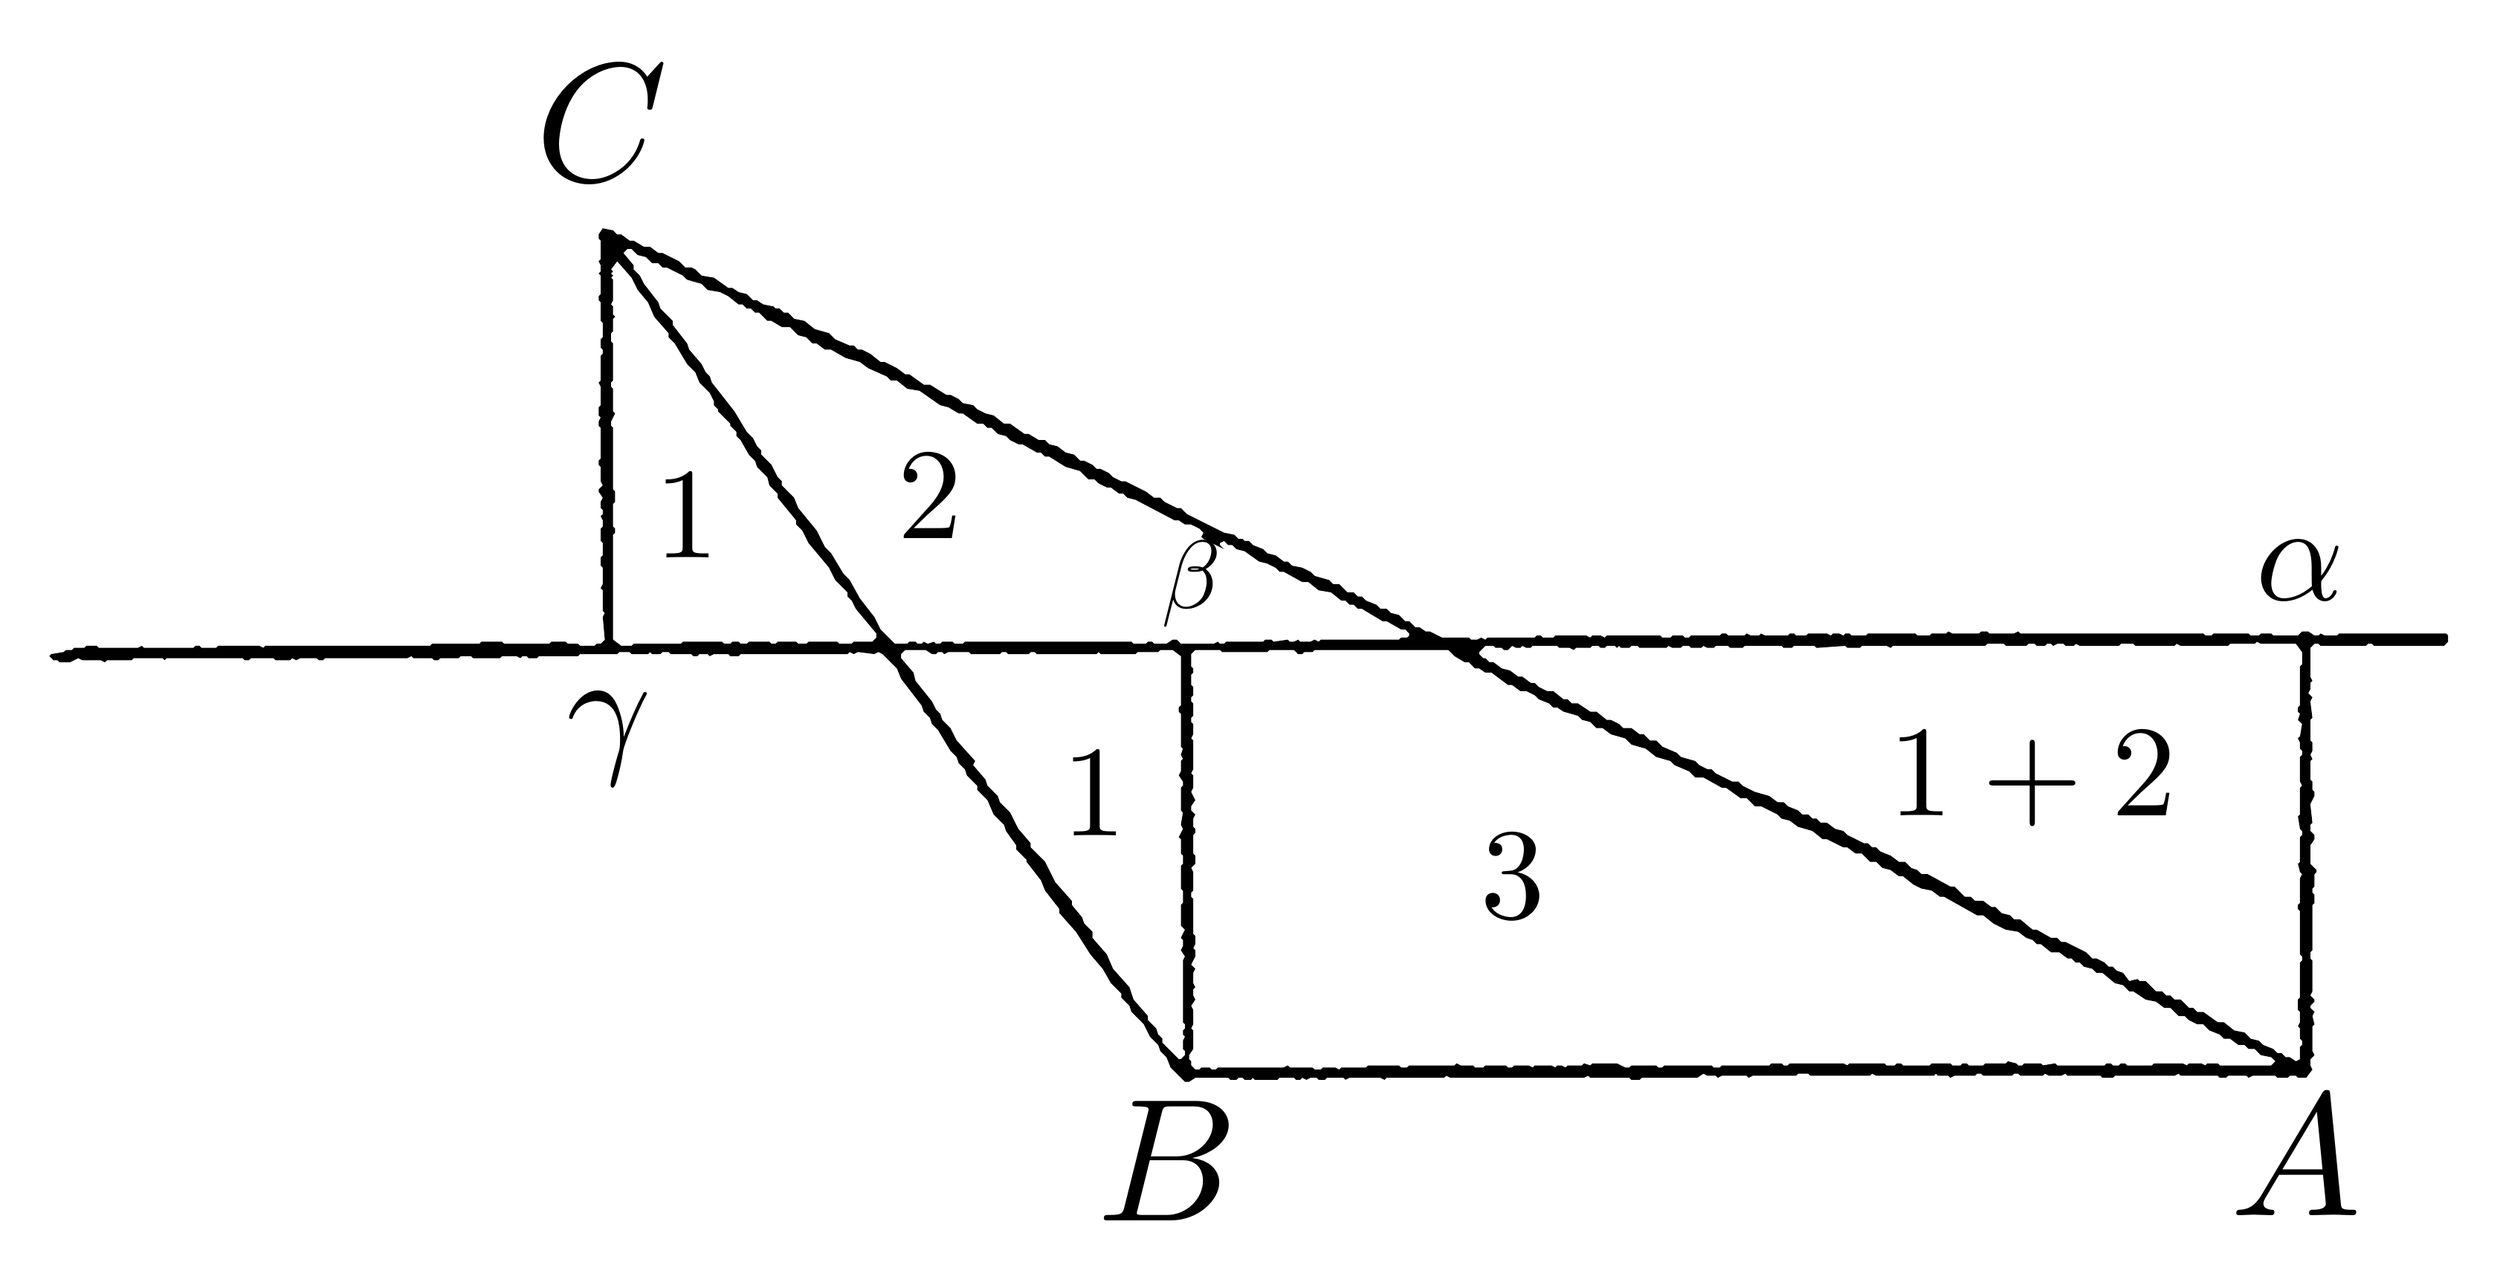
\begin{tikzpicture}[x=1pt,y=-1pt]
\path[use as bounding box] (0,0) rectangle (1195,606);
\path[fill=black,draw=none,even odd rule]
(14,309) -- (16,311) -- (18,311) -- (19,312) -- (24,312) -- (28,310) -- (30,311) -- (39,311) -- (41,312) -- (42,311) -- (54,311) -- (55,310) -- (69,310) -- (70,311) -- (71,310) -- (108,310) -- (109,311) -- (111,311) -- (112,310) -- (123,310) -- (124,311) -- (131,311) -- (132,310) -- (134,311) -- (136,310) -- (144,310) -- (145,311) -- (147,311) -- (148,310) -- (188,310) -- (190,309) -- (191,310) -- (200,310) -- (201,311) -- (203,311) -- (204,310) -- (213,310) -- (214,309) -- (219,309) -- (220,310) -- (233,310) -- (234,309) -- (241,309) -- (243,310) -- (244,309) -- (246,309) -- (247,310) -- (251,310) -- (252,309) -- (271,309) -- (272,308) -- (290,308) -- (291,307) -- (296,307) -- (297,308) -- (305,308) -- (306,307) -- (307,308) -- (311,308) -- (312,307) -- (315,307) -- (316,308) -- (326,308) -- (327,309) -- (329,309) -- (330,308) -- (334,308) -- (335,309) -- (337,308) -- (344,308) -- (345,309) -- (349,309) -- (350,308) -- (402,308) -- (403,307) -- (405,308) -- (407,307) -- (415,308) -- (417,307) -- (419,308) -- (426,315) -- (428,320) -- (438,333) -- (439,336) -- (442,339) -- (443,342) -- (446,345) -- (452,355) -- (455,358) -- (456,361) -- (459,364) -- (460,367) -- (465,372) -- (465,374) -- (470,379) -- (473,386) -- (478,391) -- (479,394) -- (484,401) -- (484,403) -- (489,408) -- (489,409) -- (496,418) -- (498,423) -- (505,432) -- (505,434) -- (513,443) -- (520,454) -- (526,461) -- (530,468) -- (535,473) -- (535,475) -- (539,479) -- (540,482) -- (546,488) -- (549,494) -- (553,498) -- (554,501) -- (557,504) -- (559,509) -- (566,516) -- (568,516) -- (571,514) -- (587,514) -- (588,515) -- (591,515) -- (592,514) -- (594,514) -- (595,515) -- (598,515) -- (599,514) -- (600,515) -- (611,515) -- (612,514) -- (619,514) -- (620,515) -- (622,515) -- (623,514) -- (625,515) -- (627,514) -- (630,514) -- (631,515) -- (634,515) -- (635,514) -- (643,514) -- (644,515) -- (646,514) -- (661,514) -- (663,515) -- (664,514) -- (692,514) -- (693,513) -- (695,514) -- (760,514) -- (762,513) -- (763,514) -- (782,514) -- (783,515) -- (787,515) -- (788,514) -- (815,514) -- (818,512) -- (820,513) -- (824,513) -- (825,514) -- (827,513) -- (839,513) -- (840,514) -- (842,513) -- (863,513) -- (864,512) -- (869,512) -- (870,513) -- (899,513) -- (900,512) -- (902,513) -- (930,513) -- (931,512) -- (932,513) -- (937,513) -- (938,514) -- (940,513) -- (950,513) -- (951,512) -- (953,512) -- (954,513) -- (968,513) -- (969,512) -- (971,512) -- (972,513) -- (983,513) -- (984,512) -- (986,513) -- (992,513) -- (994,512) -- (995,513) -- (1011,513) -- (1012,514) -- (1017,514) -- (1018,513) -- (1047,513) -- (1049,512) -- (1050,513) -- (1068,513) -- (1069,514) -- (1072,514) -- (1073,513) -- (1082,513) -- (1083,514) -- (1085,513) -- (1096,513) -- (1097,514) -- (1102,514) -- (1103,513) -- (1106,513) -- (1107,514) -- (1111,514) -- (1114,510) -- (1113,508) -- (1113,505) -- (1115,503) -- (1114,501) -- (1114,489) -- (1115,488) -- (1114,484) -- (1115,482) -- (1113,480) -- (1113,479) -- (1115,477) -- (1115,476) -- (1113,474) -- (1114,472) -- (1114,457) -- (1113,456) -- (1113,453) -- (1114,452) -- (1114,430) -- (1115,429) -- (1115,425) -- (1114,424) -- (1114,422) -- (1115,421) -- (1115,415) -- (1116,414) -- (1116,413) -- (1113,410) -- (1113,401) -- (1115,398) -- (1115,396) -- (1113,394) -- (1113,391) -- (1114,390) -- (1113,381) -- (1115,377) -- (1115,375) -- (1114,374) -- (1114,370) -- (1113,369) -- (1113,360) -- (1114,359) -- (1113,357) -- (1114,355) -- (1114,351) -- (1113,350) -- (1113,340) -- (1114,339) -- (1113,331) -- (1114,329) -- (1112,327) -- (1113,325) -- (1113,322) -- (1114,321) -- (1113,319) -- (1113,305) -- (1115,303) -- (1117,303) -- (1118,304) -- (1140,304) -- (1141,303) -- (1143,303) -- (1144,304) -- (1178,304) -- (1180,302) -- (1180,299) -- (1179,298) -- (1127,298) -- (1126,299) -- (1120,299) -- (1118,298) -- (1117,299) -- (1115,299) -- (1112,297) -- (1109,297) -- (1107,299) -- (1095,299) -- (1094,298) -- (1089,298) -- (1088,299) -- (1084,299) -- (1083,298) -- (1066,298) -- (1065,299) -- (1062,299) -- (1061,298) -- (972,298) -- (971,297) -- (969,298) -- (957,298) -- (956,297) -- (953,297) -- (952,298) -- (939,298) -- (937,297) -- (936,298) -- (929,298) -- (928,299) -- (922,299) -- (921,298) -- (898,298) -- (897,299) -- (890,299) -- (889,298) -- (887,298) -- (886,299) -- (884,298) -- (881,298) -- (880,299) -- (878,298) -- (869,298) -- (868,299) -- (863,299) -- (862,298) -- (860,298) -- (859,299) -- (848,299) -- (846,298) -- (845,299) -- (841,299) -- (839,298) -- (838,299) -- (830,299) -- (829,298) -- (827,298) -- (826,299) -- (812,299) -- (811,300) -- (809,300) -- (808,299) -- (803,299) -- (802,300) -- (798,300) -- (797,299) -- (771,299) -- (770,300) -- (768,299) -- (764,299) -- (763,300) -- (761,299) -- (746,299) -- (745,300) -- (740,300) -- (739,299) -- (737,299) -- (736,300) -- (713,300) -- (712,301) -- (710,300) -- (708,301) -- (705,301) -- (704,300) -- (691,300) -- (685,297) -- (683,297) -- (680,295) -- (678,295) -- (675,292) -- (673,292) -- (670,289) -- (666,288) -- (664,286) -- (661,286) -- (659,284) -- (654,282) -- (652,280) -- (650,280) -- (648,278) -- (645,278) -- (641,274) -- (638,274) -- (636,272) -- (629,270) -- (627,268) -- (623,266) -- (618,265) -- (616,263) -- (614,263) -- (610,260) -- (606,259) -- (604,257) -- (599,255) -- (597,253) -- (595,253) -- (594,252) -- (592,252) -- (590,250) -- (585,249) -- (567,240) -- (564,237) -- (562,237) -- (556,234) -- (554,232) -- (551,232) -- (547,229) -- (537,224) -- (535,224) -- (531,222) -- (529,220) -- (525,218) -- (523,218) -- (521,216) -- (517,214) -- (515,214) -- (512,211) -- (508,210) -- (504,207) -- (500,206) -- (498,204) -- (495,204) -- (490,201) -- (488,201) -- (481,196) -- (478,196) -- (473,192) -- (469,191) -- (465,189) -- (463,187) -- (458,186) -- (456,184) -- (452,182) -- (450,182) -- (442,177) -- (439,177) -- (432,172) -- (430,172) -- (426,169) -- (420,166) -- (418,166) -- (413,162) -- (409,160) -- (407,160) -- (405,158) -- (403,158) -- (396,155) -- (393,152) -- (386,150) -- (381,146) -- (376,145) -- (373,142) -- (371,142) -- (369,140) -- (367,140) -- (366,139) -- (361,138) -- (358,136) -- (356,136) -- (353,133) -- (349,132) -- (346,130) -- (344,130) -- (337,125) -- (331,124) -- (328,121) -- (326,120) -- (323,120) -- (320,117) -- (312,113) -- (310,113) -- (306,110) -- (303,110) -- (298,107) -- (296,107) -- (292,104) -- (290,104) -- (288,102) -- (283,101) -- (281,104) -- (281,106) -- (282,107) -- (282,116) -- (281,117) -- (282,119) -- (282,122) -- (281,123) -- (282,124) -- (282,133) -- (281,134) -- (281,136) -- (282,137) -- (282,146) -- (283,147) -- (283,154) -- (282,155) -- (282,159) -- (283,160) -- (283,162) -- (282,163) -- (282,175) -- (281,176) -- (282,178) -- (282,187) -- (281,188) -- (281,192) -- (282,193) -- (281,195) -- (281,197) -- (282,198) -- (282,213) -- (281,214) -- (281,216) -- (282,217) -- (282,224) -- (283,226) -- (281,228) -- (281,229) -- (283,232) -- (282,234) -- (282,237) -- (283,238) -- (283,240) -- (282,241) -- (283,243) -- (283,246) -- (282,247) -- (282,253) -- (283,254) -- (283,260) -- (282,261) -- (282,265) -- (283,266) -- (283,274) -- (282,276) -- (283,277) -- (283,287) -- (284,288) -- (283,290) -- (284,301) -- (282,303) -- (280,303) -- (279,304) -- (272,304) -- (271,303) -- (266,303) -- (265,302) -- (258,302) -- (257,303) -- (235,303) -- (234,302) -- (224,302) -- (223,303) -- (200,303) -- (199,304) -- (119,304) -- (118,305) -- (116,304) -- (96,304) -- (95,305) -- (88,305) -- (87,304) -- (85,304) -- (84,305) -- (60,305) -- (59,304) -- (57,305) -- (38,305) -- (37,304) -- (32,304) -- (31,305) -- (26,305) -- (25,306) -- (22,306) -- (21,307) -- (15,308) -- cycle
(569,308) -- (571,306) -- (583,306) -- (584,307) -- (606,307) -- (607,306) -- (619,306) -- (621,308) -- (623,308) -- (624,307) -- (628,307) -- (629,306) -- (694,306) -- (697,309) -- (702,312) -- (704,312) -- (707,315) -- (709,315) -- (712,317) -- (715,317) -- (723,323) -- (725,323) -- (729,326) -- (732,326) -- (736,328) -- (738,330) -- (743,332) -- (745,334) -- (747,334) -- (750,336) -- (757,338) -- (759,340) -- (763,341) -- (766,344) -- (769,344) -- (773,347) -- (780,349) -- (783,352) -- (790,354) -- (795,358) -- (802,360) -- (804,362) -- (811,365) -- (814,368) -- (818,368) -- (827,373) -- (829,373) -- (836,378) -- (839,378) -- (843,382) -- (846,382) -- (854,386) -- (856,388) -- (860,389) -- (864,392) -- (871,394) -- (876,398) -- (878,398) -- (886,402) -- (888,402) -- (892,405) -- (895,405) -- (899,409) -- (902,409) -- (905,412) -- (909,413) -- (913,416) -- (915,416) -- (920,420) -- (924,422) -- (929,423) -- (933,426) -- (935,426) -- (951,435) -- (954,435) -- (959,439) -- (965,442) -- (971,443) -- (975,446) -- (978,447) -- (980,449) -- (982,449) -- (987,453) -- (991,453) -- (995,456) -- (997,456) -- (999,458) -- (1001,458) -- (1003,460) -- (1007,461) -- (1009,463) -- (1012,463) -- (1018,468) -- (1022,469) -- (1025,472) -- (1027,472) -- (1033,476) -- (1038,477) -- (1042,480) -- (1045,480) -- (1049,484) -- (1052,484) -- (1054,486) -- (1058,488) -- (1061,488) -- (1064,491) -- (1069,493) -- (1071,495) -- (1074,495) -- (1078,498) -- (1081,498) -- (1083,500) -- (1086,500) -- (1089,503) -- (1094,504) -- (1096,506) -- (1094,508) -- (1069,508) -- (1068,507) -- (1063,507) -- (1062,508) -- (1060,507) -- (1054,507) -- (1053,508) -- (1051,507) -- (1037,507) -- (1036,508) -- (1024,508) -- (1023,507) -- (1021,507) -- (1020,508) -- (1017,508) -- (1016,507) -- (1014,507) -- (1013,508) -- (990,508) -- (989,507) -- (983,508) -- (982,507) -- (974,507) -- (973,508) -- (971,508) -- (970,507) -- (966,506) -- (965,507) -- (955,507) -- (954,508) -- (947,508) -- (946,507) -- (944,507) -- (943,508) -- (939,508) -- (938,507) -- (929,507) -- (928,508) -- (915,508) -- (914,507) -- (912,507) -- (911,508) -- (907,508) -- (906,507) -- (889,507) -- (888,508) -- (886,507) -- (860,507) -- (859,508) -- (857,508) -- (856,507) -- (851,507) -- (850,508) -- (827,508) -- (826,509) -- (823,509) -- (822,508) -- (799,508) -- (798,509) -- (796,509) -- (795,508) -- (783,508) -- (782,509) -- (780,509) -- (776,507) -- (764,507) -- (763,508) -- (760,507) -- (759,508) -- (752,508) -- (751,509) -- (749,508) -- (747,508) -- (746,509) -- (744,508) -- (736,508) -- (735,509) -- (733,508) -- (726,508) -- (725,509) -- (723,509) -- (722,508) -- (712,508) -- (711,509) -- (707,509) -- (706,508) -- (700,508) -- (698,507) -- (697,508) -- (675,508) -- (674,509) -- (671,509) -- (670,508) -- (655,508) -- (654,509) -- (642,509) -- (641,510) -- (639,509) -- (633,509) -- (632,510) -- (629,510) -- (628,509) -- (617,509) -- (616,508) -- (614,509) -- (582,509) -- (581,510) -- (579,510) -- (578,509) -- (574,509) -- (573,510) -- (571,510) -- (569,508) -- (569,506) -- (568,505) -- (568,503) -- (570,500) -- (570,491) -- (569,490) -- (570,488) -- (570,481) -- (569,479) -- (571,476) -- (570,474) -- (570,471) -- (571,470) -- (570,468) -- (570,463) -- (571,461) -- (569,459) -- (571,455) -- (571,452) -- (570,451) -- (571,449) -- (571,445) -- (570,444) -- (570,427) -- (569,426) -- (569,424) -- (570,423) -- (570,414) -- (569,412) -- (571,410) -- (571,406) -- (570,405) -- (570,396) -- (571,395) -- (571,393) -- (570,392) -- (570,388) -- (571,386) -- (569,384) -- (569,382) -- (571,379) -- (569,375) -- (570,373) -- (570,367) -- (569,366) -- (570,364) -- (570,350) -- (569,349) -- (570,347) -- (570,342) -- (569,341) -- (569,339) -- (570,338) -- (570,332) -- (569,331) -- (569,329) -- (570,328) -- (570,324) -- (569,323) -- (569,318) -- (570,317) -- (570,315) -- (569,314) -- cycle
(430,306) -- (440,306) -- (443,308) -- (445,308) -- (446,307) -- (448,307) -- (449,308) -- (451,307) -- (461,307) -- (462,308) -- (476,308) -- (477,307) -- (479,307) -- (480,308) -- (490,308) -- (491,307) -- (493,307) -- (494,308) -- (523,308) -- (524,307) -- (525,308) -- (542,308) -- (543,307) -- (553,307) -- (554,306) -- (560,306) -- (564,309) -- (564,333) -- (563,334) -- (563,336) -- (564,337) -- (564,353) -- (565,354) -- (564,357) -- (565,359) -- (564,360) -- (564,365) -- (563,367) -- (565,370) -- (565,372) -- (564,373) -- (564,384) -- (565,385) -- (564,391) -- (565,393) -- (563,397) -- (564,398) -- (564,405) -- (565,406) -- (565,410) -- (564,411) -- (564,422) -- (565,423) -- (565,429) -- (564,430) -- (564,440) -- (566,442) -- (564,446) -- (565,447) -- (565,450) -- (564,452) -- (566,455) -- (565,457) -- (565,487) -- (566,488) -- (566,490) -- (565,491) -- (565,493) -- (566,494) -- (565,496) -- (565,500) -- (566,501) -- (566,503) -- (564,505) -- (563,505) -- (555,497) -- (555,495) -- (553,493) -- (552,490) -- (548,486) -- (548,484) -- (541,476) -- (539,470) -- (531,461) -- (528,454) -- (521,446) -- (521,443) -- (517,439) -- (516,436) -- (511,430) -- (511,428) -- (503,419) -- (498,409) -- (491,402) -- (491,400) -- (485,393) -- (481,385) -- (476,380) -- (475,377) -- (470,372) -- (469,369) -- (463,362) -- (464,360) -- (455,350) -- (452,344) -- (448,340) -- (447,337) -- (445,335) -- (443,331) -- (435,321) -- (434,317) -- (428,310) -- (428,308) -- cycle
(1108,505) -- (1106,506) -- (1103,504) -- (1101,504) -- (1099,502) -- (1097,502) -- (1095,500) -- (1090,498) -- (1088,496) -- (1084,495) -- (1081,492) -- (1076,491) -- (1071,487) -- (1068,487) -- (1061,482) -- (1058,482) -- (1056,480) -- (1054,480) -- (1050,476) -- (1047,476) -- (1045,474) -- (1043,474) -- (1041,472) -- (1038,472) -- (1033,467) -- (1030,467) -- (1029,466) -- (1025,467) -- (1022,463) -- (1019,462) -- (1017,460) -- (1015,460) -- (1013,458) -- (1009,456) -- (1007,456) -- (1004,453) -- (994,448) -- (992,448) -- (990,446) -- (987,446) -- (980,442) -- (978,442) -- (972,437) -- (969,437) -- (967,435) -- (963,434) -- (960,431) -- (958,431) -- (954,428) -- (950,428) -- (948,426) -- (945,426) -- (940,421) -- (938,421) -- (927,415) -- (924,415) -- (922,413) -- (919,412) -- (916,409) -- (913,409) -- (909,406) -- (904,404) -- (902,402) -- (900,402) -- (898,400) -- (896,400) -- (888,396) -- (886,394) -- (882,393) -- (878,390) -- (875,390) -- (873,388) -- (871,388) -- (869,386) -- (866,386) -- (864,384) -- (859,382) -- (857,380) -- (854,380) -- (850,377) -- (843,375) -- (837,372) -- (835,370) -- (832,370) -- (824,366) -- (822,364) -- (820,364) -- (816,362) -- (814,360) -- (807,358) -- (805,356) -- (798,353) -- (795,350) -- (792,350) -- (789,347) -- (787,347) -- (783,344) -- (779,344) -- (777,342) -- (773,340) -- (771,340) -- (766,336) -- (763,336) -- (757,332) -- (754,332) -- (752,330) -- (750,330) -- (745,326) -- (742,326) -- (738,324) -- (736,322) -- (734,322) -- (730,319) -- (728,319) -- (724,316) -- (720,315) -- (716,312) -- (714,312) -- (712,310) -- (711,310) -- (709,308) -- (709,307) -- (712,304) -- (716,304) -- (717,305) -- (720,305) -- (721,306) -- (723,306) -- (725,304) -- (727,305) -- (729,305) -- (730,304) -- (732,305) -- (734,305) -- (735,304) -- (747,304) -- (748,305) -- (753,305) -- (755,306) -- (756,305) -- (763,305) -- (764,304) -- (767,304) -- (768,305) -- (770,305) -- (771,304) -- (775,304) -- (776,305) -- (777,304) -- (778,305) -- (782,305) -- (783,304) -- (786,304) -- (787,305) -- (800,305) -- (801,304) -- (803,305) -- (807,305) -- (808,304) -- (811,304) -- (812,305) -- (817,305) -- (818,304) -- (820,305) -- (823,305) -- (824,304) -- (830,304) -- (831,305) -- (837,305) -- (838,304) -- (856,304) -- (857,305) -- (861,305) -- (862,304) -- (872,304) -- (873,305) -- (887,304) -- (888,305) -- (894,305) -- (895,304) -- (907,304) -- (909,305) -- (910,304) -- (955,304) -- (956,303) -- (964,303) -- (965,304) -- (975,304) -- (976,303) -- (979,303) -- (980,304) -- (984,304) -- (985,303) -- (987,303) -- (988,304) -- (990,303) -- (993,303) -- (994,304) -- (998,304) -- (999,303) -- (1001,304) -- (1020,304) -- (1021,303) -- (1027,303) -- (1028,304) -- (1047,304) -- (1048,303) -- (1050,304) -- (1073,304) -- (1074,303) -- (1086,303) -- (1087,302) -- (1089,303) -- (1106,303) -- (1109,307) -- (1109,313) -- (1108,314) -- (1108,333) -- (1107,334) -- (1107,336) -- (1108,337) -- (1107,340) -- (1109,342) -- (1108,348) -- (1107,349) -- (1108,351) -- (1108,354) -- (1109,355) -- (1109,357) -- (1108,358) -- (1108,370) -- (1109,372) -- (1108,373) -- (1108,386) -- (1107,387) -- (1108,393) -- (1109,394) -- (1109,396) -- (1108,397) -- (1108,409) -- (1107,410) -- (1108,414) -- (1109,415) -- (1108,417) -- (1108,429) -- (1107,430) -- (1107,432) -- (1108,433) -- (1108,454) -- (1109,455) -- (1109,457) -- (1108,458) -- (1108,475) -- (1107,476) -- (1107,481) -- (1108,482) -- (1108,487) -- (1107,489) -- (1108,490) -- (1108,495) -- (1109,496) -- (1109,498) -- (1108,499) -- cycle
(290,117) -- (297,125) -- (300,131) -- (305,137) -- (308,144) -- (315,152) -- (315,154) -- (318,157) -- (324,167) -- (328,171) -- (330,176) -- (335,181) -- (337,185) -- (337,187) -- (339,189) -- (339,190) -- (345,196) -- (345,197) -- (348,200) -- (348,202) -- (350,204) -- (354,211) -- (357,214) -- (358,217) -- (363,222) -- (364,226) -- (368,230) -- (368,232) -- (377,243) -- (377,245) -- (380,248) -- (383,254) -- (393,266) -- (396,272) -- (402,278) -- (402,280) -- (404,282) -- (406,286) -- (416,298) -- (416,300) -- (414,302) -- (405,302) -- (404,303) -- (398,303) -- (397,302) -- (383,302) -- (382,303) -- (378,303) -- (377,302) -- (368,302) -- (367,303) -- (365,303) -- (364,302) -- (354,302) -- (353,303) -- (350,303) -- (349,302) -- (346,302) -- (345,303) -- (342,303) -- (341,302) -- (322,302) -- (321,303) -- (298,303) -- (297,304) -- (292,304) -- (288,301) -- (288,250) -- (289,249) -- (289,247) -- (288,246) -- (288,235) -- (289,234) -- (289,229) -- (288,228) -- (288,198) -- (287,197) -- (287,195) -- (289,191) -- (288,190) -- (288,179) -- (287,178) -- (287,176) -- (288,175) -- (288,157) -- (287,156) -- (287,152) -- (288,151) -- (288,145) -- (289,144) -- (288,143) -- (288,139) -- (287,138) -- (288,136) -- (288,126) -- (287,125) -- (288,124) -- (287,123) -- (288,122) -- (287,121) -- cycle
(293,113) -- (295,111) -- (297,111) -- (300,114) -- (304,115) -- (307,118) -- (310,118) -- (312,120) -- (314,120) -- (322,124) -- (324,126) -- (331,128) -- (334,131) -- (340,132) -- (344,134) -- (349,138) -- (351,138) -- (353,140) -- (355,140) -- (357,142) -- (359,142) -- (363,146) -- (365,146) -- (370,149) -- (374,149) -- (378,153) -- (382,154) -- (385,157) -- (387,157) -- (391,160) -- (394,160) -- (401,164) -- (408,166) -- (412,169) -- (421,173) -- (423,175) -- (426,175) -- (431,179) -- (437,180) -- (447,187) -- (451,188) -- (456,191) -- (458,191) -- (465,196) -- (468,196) -- (470,198) -- (472,198) -- (475,201) -- (479,202) -- (481,204) -- (485,206) -- (487,206) -- (494,210) -- (496,210) -- (498,212) -- (500,212) -- (508,217) -- (515,219) -- (519,223) -- (522,223) -- (524,225) -- (528,227) -- (530,227) -- (534,230) -- (536,230) -- (538,232) -- (542,233) -- (561,243) -- (563,243) -- (566,245) -- (569,245) -- (573,247) -- (575,249) -- (574,251) -- (575,252) -- (585,257) -- (583,255) -- (583,254) -- (585,253) -- (587,255) -- (589,255) -- (591,257) -- (595,258) -- (602,263) -- (606,264) -- (610,266) -- (612,268) -- (614,268) -- (623,273) -- (626,273) -- (631,277) -- (637,278) -- (642,282) -- (644,282) -- (646,284) -- (648,284) -- (650,286) -- (652,286) -- (662,292) -- (664,292) -- (671,296) -- (673,296) -- (675,298) -- (675,299) -- (674,300) -- (671,300) -- (670,301) -- (632,301) -- (631,302) -- (629,301) -- (627,302) -- (622,302) -- (621,301) -- (619,302) -- (617,302) -- (616,301) -- (609,302) -- (608,301) -- (605,301) -- (604,302) -- (586,302) -- (585,303) -- (583,303) -- (582,302) -- (580,303) -- (564,303) -- (562,301) -- (560,301) -- (557,303) -- (551,303) -- (550,302) -- (548,302) -- (547,303) -- (541,303) -- (540,302) -- (459,302) -- (458,303) -- (454,303) -- (453,302) -- (448,302) -- (447,303) -- (445,303) -- (444,302) -- (441,303) -- (439,302) -- (438,303) -- (436,303) -- (435,302) -- (432,302) -- (431,303) -- (425,303) -- (418,296) -- (415,290) -- (408,281) -- (403,272) -- (400,269) -- (394,259) -- (391,256) -- (387,248) -- (378,237) -- (376,232) -- (370,226) -- (370,224) -- (368,222) -- (365,216) -- (360,211) -- (360,209) -- (358,207) -- (356,203) -- (353,200) -- (347,190) -- (336,176) -- (335,173) -- (333,171) -- (331,167) -- (325,160) -- (324,157) -- (317,148) -- (317,146) -- (311,140) -- (310,137) -- (303,128) -- (301,124) -- (298,121) -- (298,119) -- cycle;
\node[inner sep=0pt,font=\fontsize{10}{10}\selectfont] at (282.5,50.0) {\scalebox{8.2}{$C$}};
\node[inner sep=0pt,font=\fontsize{10}{10}\selectfont] at (286.0,349.0) {\scalebox{7.2}{$\gamma$}};
\node[inner sep=0pt,font=\fontsize{10}{10}\selectfont] at (569.0,274.0) {\scalebox{4.7}{$\beta$}};
\node[inner sep=0pt,font=\fontsize{10}{10}\selectfont] at (1108.0,267.5) {\scalebox{6.7}{$\alpha$}};
\node[inner sep=0pt,font=\fontsize{10}{10}\selectfont] at (324.0,241.0) {\scalebox{6.3}{$1$}};
\node[inner sep=0pt,font=\fontsize{10}{10}\selectfont] at (442.0,231.5) {\scalebox{6.3}{$2$}};
\node[inner sep=0pt,font=\fontsize{10}{10}\selectfont] at (522.0,376.0) {\scalebox{6.3}{$1$}};
\node[inner sep=0pt,font=\fontsize{10}{10}\selectfont] at (725.5,416.0) {\scalebox{6.3}{$3$}};
\node[inner sep=0pt,font=\fontsize{10}{10}\selectfont] at (978.0,369.0) {\scalebox{6.3}{$1+2$}};
\node[inner sep=0pt,font=\fontsize{10}{10}\selectfont] at (557.5,554.5) {\scalebox{8.5}{$B$}};
\node[inner sep=0pt,font=\fontsize{10}{10}\selectfont] at (1106.0,552.0) {\scalebox{8.5}{$A$}};
\end{tikzpicture}%
}
\end{center}

I do not have time now to write everything out in full textbook form, but what I have said will suffice to make the essence of the synthetic proof \mbox{clear. \mbox{.\,.\,.}}

\medskip

\Needspace{7\baselineskip}
\begin{center}
REMARK.
\end{center}

\textsc{Gauss} also noted down the preceding proof in a notebook under the same title as the letter extracts here. Exactly the same proof had already been given in 1836 by \textsc{Lobachevsky} in \S\,68 of the paper \gausscyr{Новыя начала геометріи} (New principles of geometry).

\begin{flushright}
\textsc{Stäckel}.
\end{flushright}
%
\clearpage\SourceLeaf{302}
\begin{center}
\textbf{[ON MÖBIUS'S BARYCENTRIC CALCULUS.]}

\medskip

[I.]
\end{center}

\begin{center}\textsc{Gauss} to \textsc{Schumacher}. Göttingen, 12 May 1843.\end{center}

I still owe you my thanks, my dearest friend, for several of your letters and other
interesting communications. But you must not keep too strict an account with
me. For 4---6 weeks I have been drawn into some
mathematical speculations (at first by chance circumstances), in which new prospects
have repeatedly led me in different directions. I have achieved much and missed much. Amid
such wandering one is (or at least I am) almost incapable of taking up any
other subject, and so my correspondence in particular has fallen very far behind.
Those speculations have mostly concerned carrying through methods of my own
rather than new matters. Most recently they have concerned, among other things, several
questions about conics. This has reminded me that half a
century ago, when I first read \textsc{Newton}'s Principia, I found several things
unsatisfactory, especially his propositions on conics, admirable in themselves.
Yet I always read with the feeling that what I had learned did not give me command of the
subject. I was particularly troubled by the straight line by means of which a conic
can be described. \textsc{Newton} solves the problem of drawing a conic through 5 points $A$, $B$,
$C$, $D$, $E$ by first using the four
%
\SourceLeaf{303}%
points $A$, $B$, $C$, $D$ (I am using my own notation here, as I find \textsc{Newton}'s
rather cumbersome in this case) to find a point $\delta$ on that straight line.
He then uses $A$, $B$, $C$, $E$ to find another point $\varepsilon$ on the
line. The straight line itself is thus given in position, and for any other
point on it, $\mu$, his construction gives a corresponding
point $M$ on the conic. He lets the angle $BAC$ (with arms of unspecified length)
rotate about $A$ and notes the position in which $AB$ passes through $\mu$. Then $AC$ must
pass through $M$. Likewise, when the angle $ABC$ rotates about $B$, as
$BA$ passes through $\mu$, $BC$ must also pass through $M$. This construction is
exceedingly elegant, but one has command of the subject only when one can answer
all the other questions concerning this magical straight line.
In particular, one wants to know what relations this straight line has to the elements of the
conic, and whether those elements can themselves be derived easily from the position of the
straight line and the positions of $A$, $B$, $C$. I can now handle several things of this kind
quite elegantly, but I do not know whether I can carry the whole matter through myself,
since other duties force me to break off.

\mbox{.\,.\,.\,.\,.\,.\,.} Formerly, if I am not mistaken, you spent much time on conics.
You have certainly read much more on them than I have. For example, already in
Monatliche Correspondenz, 1810 November, p. 508, you cite an elegant proposition about the ellipse
from a book\HistoricalNote{[*)]}{[*)}{\textsc{Puissant}, Recueil de diverses propositions de géométrie. Paris 1801.
See also vol. IV, p. 396.]} that I have not yet consulted, although our library presumably
owns it. It is therefore natural to ask you first for historical information.
Do you know an elegant construction by which the \textls{center}
of a conic from 5 of its points --- \textls{without any unnecessary detours} --- may be
found? It certainly cannot be difficult, but this is precisely the derivation I have not yet
\mbox{worked out. .\,.\,.\,.\,.\,.\,.}
%
\SourceLeaf{304}
\Needspace{6\baselineskip}\begin{center}\textsc{Gauss} to \textsc{Schumacher}. Göttingen, 15 May 1843.\end{center}

I add a few words to my last letter to you, my dearest friend,
to do justice to a book to which, partly because of a circumstance
you brought about twenty years ago (quite innocently, of course),
I have so far paid less attention than it deserves.

You may still remember that in your house at the time you presented me with a rather
elegant geometrical problem posed by \textsc{Möbius}, for which I
almost immediately wrote down a solution that left nothing to be desired. As a result
of this incident, I took up \textsc{Möbius}'s book, barycentrischer Calcul,
in whose preface that problem was also mentioned, with a kind of prejudice.
I doubted whether it was worth the trouble to master a rather ingeniously
devised method of calculation if it could achieve nothing that could not
be achieved just as easily without it. I had therefore laid the
book aside for the time being --- especially since I received it when other things
fully occupied me --- and, as has happened to me with many things, had expected little
of it and later forgotten it altogether.

In the last few days (yesterday, to be exact) I happened to come across the book,
and I soon found with great pleasure that it contains the quintessence
of the theory of conics in a nutshell, and that his
barycentric calculus leads by the easiest route to the solution of all the relevant
problems. While leafing through it, I found much else of interest as well,
for example the beautiful theorem discovered by \textsc{Mac Laurin} and \textsc{Brackenridge},
which I had either never known or forgotten again. By means of it
the problem of drawing a conic through 5 given points can be solved so
elegantly.
%
\par\SourceLeaf{305}
\indent In general, with any new calculus of this kind, whatever can be accomplished with it
can also be accomplished without it. The advantage, however, is
that if such a calculus corresponds to the very nature of frequently recurring
needs, anyone who has mastered it completely can, even without the
almost unconscious inspirations of genius, which no one can \textls{force}, solve the
problems in question, and can even solve them almost mechanically in cases so complicated
that, unaided in this way, even genius is powerless. This is true of
the invention of calculation with letters in general. It was true of differential calculus,
and it is true as well (though in more limited domains) of \textsc{Lagrange}'s
calculus of variations, my calculus of congruences, and \textsc{Möbius}'s calculus. By
such conceptions, countless problems which would otherwise stand isolated and
demand fresh efforts (smaller or greater) of inventive thought each time
form, as it were, an organic realm. \mbox{.\,.\,.\,.\,.\,.\,.\,.\,.}

\Needspace{9\baselineskip}\begin{center}
\medskip

[II.]

\textbf{[THE BARYCENTRIC CALCULUS AND THE CALCULUS OF RESULTANTS.]}

[1.]
\end{center}

The barycentric calculus has its counterpart in another (presumably even
more comprehensive) calculus that might be called the calculus of resultants. The first deals
with points at which ponderable masses are assumed. The second would deal
with lines along which forces act. If $a$, $b$, $c$,
$d$, etc. are lines along each of which forces act in a definite direction, with magnitudes
proportional to the numbers $\alpha$, $\beta$, $\gamma$, $\delta$, etc., then
the equation

\[
\alpha a + \beta b + \gamma c + \delta d + \text{etc.} = 0
\]
\noindent would mean that these forces balance one another.
%
\SourceLeaf{306}
\Needspace{5\baselineskip}\begin{center}
[2.]
\end{center}

If $B, C$ are two points on $a$, one may quite properly set $B - C = ai$.

\Needspace{5\baselineskip}\begin{center}
[3.]
\end{center}

The main question now is what forces should be applied to the vertices of the pentagon in the barycentric calculus or to its sides in the calculus of resultants, so that the relations between those forces and their equivalents on the inner pentagon are as simple as possible.

\Needspace{5\baselineskip}\begin{center}
[4.]
\end{center}

The collinearity of two systems of points or straight lines is perhaps best defined by the fact that one and the same linear equation can always be set up between any 5 points (lines) of one system and the 5 corresponding ones of the other.

\Needspace{5\baselineskip}\begin{center}
[5.]
\end{center}

The characteristic feature of a collineation seems to be most simply expressed as follows.

Let $A, B.\,.\,.$ be straight lines and $P,Q.\,.\,.$ points, all in one system, corresponding in the other to the lines $a,b.\,.\,.$ and the points $p,q.\,.\,.$. If $PA$ denotes the (perpendicular) distance of the point $P$ from the straight line $A$, then in general
\[
\frac{PA.QB.pb.qa}{pa.qb.PB.QA} = 1.
\]
%
\SourceLeaf{307}
\Needspace{8\baselineskip}\begingroup\small
\begin{center}
REMARKS.
\end{center}

The note \emph{Zur Theorie der Kegelschnitte} relates to the investigations mentioned in the letter of 12 May 1843. It is printed from the posthumous papers in the following division, Verwendung complexer Grössen für die Geometrie, on pp. 341 to 344 of this volume.

\textsc{Gauss}'s solution to the geometrical problem posed by \textsc{Möbius} was published by \textsc{Schumacher} in Astronomische Nachrichten, no. 42, 1823 November. It is reprinted in vol. IV, pp. 406---407.

Note [II] is on a separate leaf. It probably dates from the same time as the letter excerpts printed under [I]. \textsc{Gauss} applied the barycentric calculus in particular to the theory of the pentagon, as indicated under [3]. The developments in question, which are connected with the Pentagramma mirificum, can be found under the title \emph{Weitere Fragmente über das Pentagramma mirificum}, no. 11, pp. 109 to 111 of this volume (see also the accompanying remarks by \textsc{Fricke}, p. 117). See also the note \emph{Beziehung der Raumverhältnisse auf ein gegebenes Tetraeder}, vol. II, pp. 307 to 308. It probably dates from as early as July 1831.

\begin{flushright}
\textsc{Stäckel}.
\end{flushright}
\par\endgroup
%
\end{document}
